% chapter3.tex -- en (English)
\chapter{Installation and Configuration}

This chapter describes the installation of the operating system and of
all parts of the software. The main focus is on implementing a toolchain
to compile the open source software {\audacious} on the {\RPi}.

{\begin{bclogo}[arrondi = 0.2, logo = \bcdanger, ombre = true, epOmbre = 0.25, couleurOmbre = red!75,blur]{Danger!}
Some of the actions described here require opening the housing of the 
{\Bezeichnung} to reach the SD card of the built-in {\RPi}. To avoid 
dangerous electric shocks when handling inside the device, the mains 
plug must be disconnected before opening! 
\end{bclogo}

\begin{bclogo}[logo = \bclampe, noborder = true]{Hint}
This tutorial was tested on a {\RPi} running \cmd{Linux raspiblaster 
4.14.30-v7+ \#1102 SMP Mon Mar 26 16:45:49 BST 2018 armv7l GNU/Linux}.

The PC commands differ depending on the used operating system (Linux or
Windows). The differences are described when they occur.
\end{bclogo}


In this manual a lot of commands have to be started either on the {\RPi}
or on a PC in a terminal window. To copy data from the PC to the
{\Bezeichnung} both computers must be connected via LAN (or WLAN). The
data exchange is done via \textit{ssh (\textbf{s}ecure 
\textbf{sh}ell)}.\\
Instead of entering all commands on the {\RPi} via a second keyboard it
is useful to open a terminal window on the PC and to initiate a 
\textit{ssh} connection for doing all keyboard entries on the PC. 
Another big advantage is that you can open this pdf file on your PC, 
mark the {\RPi} commands and insert them via \textit{copy+paste} into
the ssh terminal.\\
Only the first part of this tutorial (``raspi-config'') can't executed
\textit{remote} because \textit{ssh} has to be enabled on the {\RPi}
using this command first.

\begin{bclogo}[logo = \bclampe, noborder = true]{Hint}
On a Windows PC \textit{ssh} isn't installed by default. Install the 
software \textit{PuTTY} to circumvent this. You may download it from
\url{https://putty.org/}:\\
\url{https://www.chiark.greenend.org.uk/~sgtatham/putty/latest.html}

To connect from Windows via \textit{ssh} to the {\RPi} call the Windows 
start menu item \mbox{``PuTTY64''}. To log in you will need the IP
address of the {\RPi} and the user \cmd{pi} and its password (see 
figures \ref{fig:putty01} und \ref{fig:putty02}). 
\end{bclogo}

\begin{figure}[h]
\centering
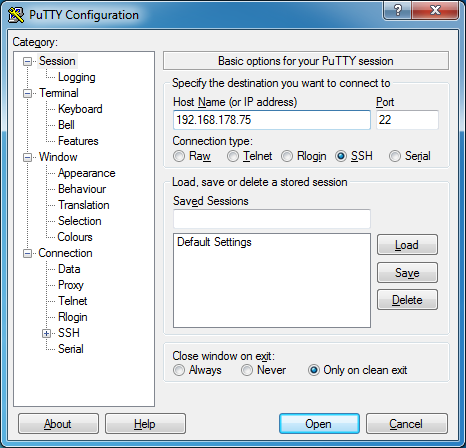
\includegraphics[width=0.5\textwidth]{putty01.png}
\caption{Connect from Windows PC to {\RPi} via \textit{PuTTY}}
\label{fig:putty01}
\end{figure}

\begin{figure}[h]
\centering
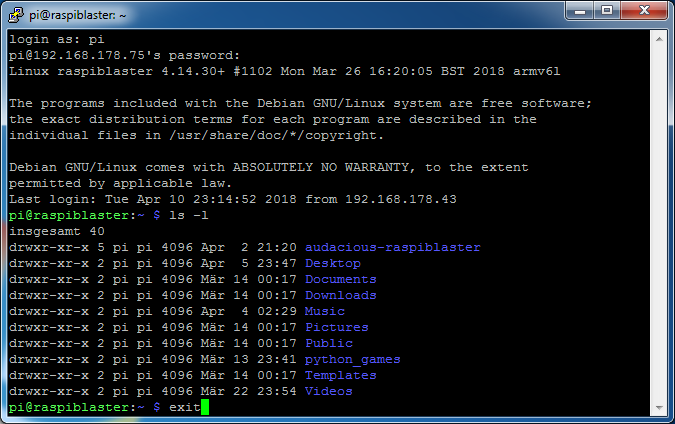
\includegraphics[width=0.75\textwidth]{putty02.png}
\caption{\textit{PuTTY} remote console of {\RPi} on the Windows PC}
\label{fig:putty02}
\end{figure}


\newpage
\section{Configure Raspbian}
\subsection*{raspi-config}
\cmdPi{sudo raspi-config}\\
\stdout{1 Change User Password \ \ \ \ \ \ \ \ \ \ \ \ \ \ \ \ \ \ \ \ \ \ \ \ \ \ \ }\comment{\eg "raspiBlaster"}\\
\stdout{2 Network Options \ \ \ \ \ --> N1 Hostname \ \ \ \ \ \ \ \ \ \ \ \ }\comment{"raspiblaster"\ instead of "raspberrypi"}\\
\stdout{4 Localisation Options --> I1 Change Locale}\\
\stdout{\textcolor{white}{......................} --> I2 Change Timezone}\\
\stdout{\textcolor{white}{......................} --> I3 Change Keyboard Layout}\\
\stdout{\textcolor{white}{......................} --> I4 Change Wi-fi Country }\comment{really important adjustmen!}\\
\stdout{5 Interfacing Options \ --> P2 SSH}

\subsection*{Update the System}
\cmdPi{sudo apt update }\comment{update of apt meta data}\\
\cmdPi{sudo apt upgrade}\comment{upgrade of all installed packages}\\
\cmdPi{sudo apt update }\comment{sometimes necessary, \eg when using Raspbian image from 13-03-2018}\\

\subsection*{Shrink Down Image to approx. 6,8GB}
TODO:\todo{describe either my way or \cmd{pishrink} by @framp}

This step isn't mandatory but it serves two advantages:
\begin{compactitem}
\item{The image is small enough to fit on \textit{any} 8GB SD card}
\item{The time for backing up and flashing SD cards is reduced significantly}
\end{compactitem}

\subsection*{Orientation of the original \raspidisplay}
The graphics orientation should be rotated by 180� due to a better 
viewing angle. Add the line \cmd{lcd\_rotate=2} in the file 
\filenam{/boot/config.txt}.

\cmdPi{sudo nano /boot/config.txt}\\
\editor{lcd\_rotate=2}

\subsection*{Adjustment of the Raspbian PIXEL desktop}
\uline{Adjust look and feel:} \comment{depending on personal preferences}\\
Menu item \menuitem{\rpiIcon$\rightarrow$Preferences$\rightarrow$Appearance Settings: Tab 'Desktop'}\\
Checkbox \checkbox{Wastebasket}: disable \comment{cildren don't need this}\\
Combobox \combobox{Layout}{Centre image on screen}\\
Combobox \combobox{Picture}{raspberry-pi-logo.png} \comment{use the raspberry pi logo on the desktop}

\uline{Reduce Duble Click Speed for Touch Screen Operating:}\\
Menu item \menuitem{\rpiIcon$\rightarrow$Preferences$\rightarrow$Mouse and Keyboard Settings: Tab 'Mouse'}\\
Slider \checkbox{Double-click Delay}: \cmd{1990}ms \comment{the default of 250ms is too short for a touch display}

\uline{Disable Screen Saver:} \comment{Optional!}\\
add the following line at section \cmd{[Seat: *]}:

\cmdPi{sudo nano /etc/lightdm/lightdm.conf}\\
\editor{[Seat: *]\\xserver-command=X -s 0 -dpms}


\section{Install HiFiBerry MiniAMP}
\uline{Resources:}\\
\url{https://www.hifiberry.com/shop/boards/miniamp}\\
\url{https://www.hifiberry.com/build/documentation/configuring-linux-3-18-x}\\
\url{https://support.hifiberry.com/hc/en-us/articles/205377202-Adding-software-volume-control}

\begin{bclogo}[logo = \bclampe, noborder = true]{Hint}
Use the drivers of HiFiBerry DAC for HiFiBerry MiniAMP V1.0!
\end{bclogo}

\subsection*{adjust \filenam{/boot/config.txt}}
Remove the entry for the on board audio module (HDMI and 3,5mm jack):\\
The entry \cmd{dtparam=audio=on} must be deleted or marked as comment,\\
use the "Device Tree Overlay File" for MiniAMP instead:

\newpage
\cmdPi{sudo nano /boot/config.txt}\\
\editor{\#dtparam=audio=on\\\vdots\\dtoverlay=hifiberry-dac}

\subsection{Configure ALSA in the file \filenam{/etc/asound.conf}}
\begin{bclogo}[logo = \bclampe, noborder = true]{Hint}
Please check first if the file \filenam{.asoundrc} exists in  the home
directory of user \cmd{pi}. This file contains user-specific ALSA 
settings and overrides the settings in \filenam{/etc/asound.conf}!
\end{bclogo}
\cmdPi{rm /home/pi/.asoundrc}

\uline{Contents of \filenam{/etc/asound.conf}:}\\
\cmdPi{cat /etc/asound.conf}\\
\stdout{pcm.!default \{}\\
\stdout{\ \ type hw card 0}\\
\stdout{\}}\\
\stdout{ctl.!default \{}\\
\stdout{\ \ type hw card 0}\\
\stdout{\}}

\cmdPi{reboot}\\
\cmdPi{aplay -l}\\
\stdout{**** List of PLAYBACK Hardware Devices ****}\\
\stdout{\smaller{card 0: sndrpihifiberry [snd\_rpi\_hifiberry\_dac], device 0: HifiBerry DAC HiFi pcm5102a-hifi-0 []}}\\
\stdout{\ \ Subdevices: 0/1}\\
\stdout{\ \ Subdevice \#0: subdevice \#0}

\subsection{Enhance ALSA for Volume Control}
\uline{Additional Contents of \filenam{/etc/asound.conf}:}\\
\cmdPi{cat /etc/asound.conf}\\
\stdout{\# Settings of @smutbert from the German Raspberry Pi forum:}\\
\stdout{\# \url{https://forum-raspberrypi.de/user/21740-smutbert/}}\\
\stdout{pcm.dmixer \{}\\
\stdout{    type dmix}\\
\stdout{    ipc\_key 1236}\\
\stdout{    slave.pcm "hw:sndrpihifiberry"}\\
\stdout{\}}\\
\stdout{pcm.softvolume \{}\\
\stdout{    type softvol}\\
\stdout{    slave.pcm "dmixer"}\\
\stdout{    control.name "Master"}\\
\stdout{    control.card sndrpihifiberry}\\
\stdout{\}}\\
\stdout{pcm.!default \{}\\
\stdout{    type       plug}\\
\stdout{    slave.pcm  "softvolume"}\\
\stdout{\}}

23-03-2018 TODO:\todo{Check why this doesn't work with omxplayer\dots}\\
@smutbert's \filenam{/etc/asound.conf} doesn't work on Raspbian Stretch 
2018-03-13 with \mbox{omxplayer}: Playback of media file stops immediately at 
0:00!\\
\stdout{\# Old Contents:}\\
\stdout{\#\#pcm.!default \{}\\
\stdout{\#\# type hw card 0}\\
\stdout{\#\#\}}\\
\stdout{\#\#ctl.!default \{}\\
\stdout{\#\# type hw card 0}\\
\stdout{\#\#\}}\\
\stdout{\#}\\
\stdout{\#pcm.hifiberryMiniAmp \{}\\
\stdout{\#    type softvol}\\
\stdout{\#    slave.pcm "plughw:0"}\\
\stdout{\#    control.name "Master"}\\
\stdout{\#    control.card 0}\\
\stdout{\#\}}\\
\stdout{\#pcm.!default \{}\\
\stdout{\#    type       plug}\\
\stdout{\#    slave.pcm  "hifiberryMiniAmp"}\\
\stdout{\#\}}

\cmdPi{rm /home/pi/.asoundrc}\\
\cmdPi{reboot}\\
\cmdPi{speaker-test -c 2}\comment{speaker-test -D hifiberryMiniAmp -c 2}\\
\cmdPi{alsamixer}

\begin{figure}[h]
\centering
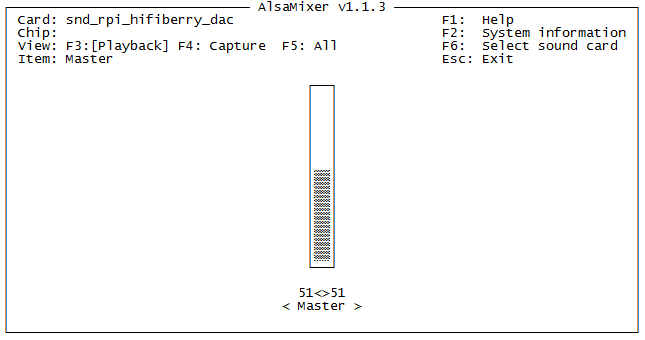
\includegraphics[width=\textwidth]{\lang/alsamixer.png}
\caption{alsamixer, a console mixing tool}
\label{fig:alsamixer}
\end{figure}

\newpage
\textit{alsamixer} shows the control \textit{Master} which is defined in
the file \filenam{/etc/asound.conf}.
\begin{bclogo}[logo = \bclampe, noborder = true]{Hint}
Volume control is done now by ALSA!\\
\textit{alsamixer} adjusts the same audio setting as the graphical 
volume control in the taskbar of Raspbian Desktop PIXEL.
\end{bclogo}

\uline{Test:}\\
\cmdPi{omxplayer -o alsa "01 Saga - Wind Him Up.wav"}


\section{Start Up the {\CDROM} Drive on the {\RPi}}
When an audio CD is inserted into the external {\CDROM} drive (resp. DVD
burner) its contents is \textit{not} mounted at \filenam{/media/pi/<volume>}!
Rather, a virtual(?) folder (or URL) is opened: 
\cmd{cdda://sr0/}\\
Direct file access to this mount path is not available and even the 
\textit{omxplayer} can't do here any magic!\\
\textbf{$\Rightarrow$ We'll need a software CD player!}

\newpage
\subsection{Detecting the External {\CDROM} drive on the USB port}
\cmdPi{lsusb}\comment{{\CDROM} drive isn't connected to USB}\\
\stdout{\smaller{Bus 001 Device 003: ID 0424:ec00 Standard Microsystems Corp. SMSC9512/9514 Fast Ethernet Adapter}}\\
\stdout{\smaller{Bus 001 Device 002: ID 0424:9514 Standard Microsystems Corp. SMC9514 Hub}}\\
\stdout{\smaller{Bus 001 Device 001: ID 1d6b:0002 Linux Foundation 2.0 root hub}}\\
\cmdPi{lsusb}\comment{{\CDROM} drive is connected}\\
\stdout{\smaller{\textcolor{darkblue}{Bus 001 Device 006: ID 0e8d:1887 MediaTek Inc.}}}\\
\stdout{\smaller{Bus 001 Device 003: ID 0424:ec00 Standard Microsystems Corp. SMSC9512/9514 Fast Ethernet Adapter}}\\
\stdout{\smaller{Bus 001 Device 002: ID 0424:9514 Standard Microsystems Corp. SMC9514 Hub}}\\
\stdout{\smaller{Bus 001 Device 001: ID 1d6b:0002 Linux Foundation 2.0 root hub}}

\subsection{Installation of Linux Package \textit{eject}}
\label{sect:eject}
For software-controlled opening of the CD tray the software package
\textit{eject} is necessary which isn't installed in Raspbian by 
default:

\cmdPi{sudo apt install eject}\comment{49,5kB archives, 225kB disk space uncompressed}\\
\cmdPi{eject \ \ }\comment{Opening of {\CDROM} drive}\\
\cmdPi{eject -t}\comment{Closing of {\CDROM} drive: Not supported by each drive type!}

%\begin{bclogo}[logo = \bclampe, noborder = true]{Hint}
The call of \cmd{eject -t} can be used anyway to check on drives which
don't support this feature, if its tray \textbf{is} opened or closed.
When the tray is open \cmd{eject -t} gives an error message and exits 
with return code 1.
%\end{bclogo}

Despite the \cmd{man} page documentation the command \cmd{eject -i 1} 
\textbf{does not} prevent the drive (at least the used drive {\LGdrive})
from ejecting the tray when pressing the eject push button. The same
behaviour can be found on my laptop computer.


\section{Compile \textit{audacious} on the {\RPi}}
\label{sect:compile}
Initial tests using several audio players resulted in dogged hanging ups 
when pressing the eject push button during playback of an audio CD. It 
didn't matter which audio player software was used. Even the command
\cmd{sudo kill -9 <process ID>} coundn't terminate the hanging 
process!\\
The first try was to prevent the CD tray from opening via the command
\cmd{eject -i 1}. But as mentioned in the preceding chapter (section
\ref{sect:eject}) this command doesn't work at least on the used drive
\LGdrive. So the circuitry at the eject push button was opened and can 
be closed via a relay contact. This ``eject lock'' can be controlled by
hardware via the GPIO pin 4.\\
So it was necessary to implement the eject lock logic into the used 
audio player software and in addition a software eject button which
performs a playback stop before. The source code had to be adjusted and
recompiled.


\subsection{Download and Uncompressing of the Current Source Code}
At first the version {\audaciousStable} of the {\audacious} source code 
was downloaded. It consists of three sub projects as compressed 
\cmd{tar} archives, so-called \textit{tar balls}:
\begin{compactitem}
\item{\cmd{libaudclient-3.5-rc2.tar.bz2}}
\item{\cmd{audacious-3.9.tar.bz2}}
\item{\cmd{audacious-plugins-3.9.tar.bz2}}
\end{compactitem}

\uline{Resources:}\\
\url{https://audacious-media-player.org/download}

\url{https://distfiles.audacious-media-player.org/libaudclient-3.5-rc2.tar.bz2}\\
\url{https://distfiles.audacious-media-player.org/audacious-3.9.tar.bz2}\\
\url{https://distfiles.audacious-media-player.org/audacious-plugins-3.9.tar.bz2}

Assuming that the download was performed on a Linux PC the three tar 
balls must be copied via \textit{ssh} onto the {\RPi} into the directory
\cmd{/home/pi/audacious\_raspiblaster}:

\cmdPi{cd /home/pi}\\
\cmdPi{mkdir audacious\_raspiblaster}

\cmdPC{scp *.tar.bz2 pi@raspiblaster:/home/pi/audacious\_raspiblaster}\\
The PC requests for the password of user \cmd{pi} on the remote host
\cmd{raspiblaster} before transferring the files via \textit{ssh} 
protocol from the PC to the {\RPi}.

\begin{bclogo}[logo = \bclampe, noborder = true]{Hint}
On a Windows PC with installed \textit{ssh} software package 
\textit{PuTTY} the command in the Windows' console terminal is
(\cmd{cmd.exe}):\\
\cmdWin{\textcolor{red}{\textbf{p}}scp *.tar.bz2 pi@raspiblaster:/home/pi/audacious\_raspiblaster}
\end{bclogo}

\uline{Unpacking the tar balls:}\\
\cmdPi{cd audacious\_raspiblaster}\\
\cmdPi{tar -xvf audacious-3.9.tar.bz2}\\
\cmdPi{tar -xvf audacious-plugins-3.9.tar.bz2}\\
\cmdPi{tar -xvf libaudclient-3.5-rc2.tar.bz2}


\subsection{Compilation of libaudclient-3.5-rc2}
\cmdPi{cd /home/pi/audacious\_raspiblaster/libaudclient-3.5-rc2}\\
\cmdPi{./configure}

The command \cmd{./configure} checks that several necessary software 
packages aren't installed yet:\\
\cmdPi{sudo apt install libglib2.0-dev \ \ \ }\comment{message: Cannot find Glib2!\\If you are using binary packages based system, check that you have the corresponding -dev/devel \mbox{packages} installed.}\\
\cmdPi{sudo apt install libdbus-1-dev \ \ \ \ }\comment{message: No package 'dbus-1' found}\\
\cmdPi{sudo apt install libdbus-glib-1-dev}\comment{message: No package 'dbus-glib-1' found}\\
\cmdPi{./configure}\\
\cmdPi{make}\comment{issues a lot of warning, but it compiles the project completely\dots}\\
\cmdPi{sudo make install}


\subsection{Compilation of audacious-3.9}
\cmdPi{cd /home/pi/audacious\_raspiblaster/audacious-3.9}\\
\cmdPi{leafpad INSTALL}\comment{shows an installation procedure}\\
\cmdPi{./configure}

The command \cmd{./configure} checks that several necessary software 
packages aren't installed yet:\\
\cmdPi{sudo apt install libglib2.0-dev \ \ \ \ \ \ \ \ }\comment{message: No package 'glib-2.0' found}\\
\cmdPi{sudo apt install libgtk2.0 libgtk2.0-dev}\comment{message: No package 'gtk+-2.0' found\\$\rightarrow$Installation of these packages takes about 5 minutes on an {\RPi} 3B}

\cmdPi{./configure}\\
\cmdPi{make -j4}\comment{\cmd{-j4} forces \texttt{make} to use all the four cores of the {\RPi} 3B}\\
\cmdPi{sudo make install}

Due to the graphical user interface of {\audacious} the next command has
to be entered on the {\RPi} itself. It can't be done on the \textit{ssh}
terminal of the PC!\\
\cmdPi{audacious}
%# liefert Fehlermeldung: audacious: error while loading shared libraries: libaudcore.so.5: cannot open shared object file: No such file or directory
%--> Wieder ein echtes Schmankerl:
%    Die "shared libraries" werden offenbar in /usr/lib gesucht und es hat nichts
%    mit dem Inhalt der PATH-Variablen zu tun!
%    "make install" kopiert die Libraries jedoch nach /usr/local/lib.
%    Abhilfe: 
%    \cmdPi{sudo cp  /usr/local/lib/* /usr/lib}
%
%\cmdPi{audacious}
%--> Jetzt erscheint eine vers�hnlichere Meldung:
%    ERROR plugin-init.cc:147 [start_required]: No output plugin found.
%    (Did you forget to install audacious-plugins?)
%    Abgebrochen
 

\subsection{Compilation of audacious-plugins-3.9}
\cmdPi{cd /home/pi/audacious\_raspiblaster/audacious-plugins-3.9}\\
\cmdPi{./configure}

The command \cmd{./configure} checks that several necessary software 
packages aren't installed yet:\\
\cmdPi{sudo apt install libxml2-dev}\comment{message: No package 'libxml-2.0' found}

A further call of \cmd{./configure} requests the libcdio library which is necessary for CD playback:\\
\textit{checking for libcdio >= 0.70 libcdio\_cdda >= 0.70 libcddb >= 1.2.1... no\\configure: WARNING: audio CD support disabled due to missing dependency: libcdio >= 0.70 libcdio\_cdda >= 0.70 libcddb >= 1.2.1}\\
\cmdPi{sudo apt install libcdio-dev libcdio-paranoia-dev libcddb-dev}

Further the flac codec is missing (which is IMHO more important than many other codecs like MP3):\\
\textit{checking for flac >= 1.2.1... no\\configure: error: Missing dependency for FLAC support: flac >= 1.2.1}

\cmdPi{sudo apt install libflac-dev}\\
\cmdPi{sudo apt install libogg-dev libvorbis-dev}\comment{ditto for codecs ogg vorbis}\\
\cmdPi{sudo apt install libfluidsynth-dev \ \ \ \ \ \ }\comment{ditto for MIDI-Plugin}\\
\cmdPi{sudo apt install libmpg123-dev \ \ \ \ \ \ \ \ \ \ }\comment{ditto for MP3-Codec}\\
\cmdPi{sudo apt install libfaad-dev \ \ \ \ \ \ \ \ \ \ \ \ }\comment{ditto for AAC-Codec}\\
\cmdPi{sudo apt install libwavpack-dev \ \ \ \ \ \ \ \ \ }\comment{ditto for WAV-Codec}\\
\cmdPi{\# sudo apt install libsamplerate-dev \ \ \ \ }%\comment{necessary for plugin Speed+Pitch: Funny for children and adults}

\uline{Installation of package neon27 fOr HTTP/HTTPS Transport:}\\
\cmdPi{sudo apt install libneon27-dev}

\uline{Ugly warning: ALSA is mandatory on {\Bezeichnung} for audio playback!}\\
\textit{checking for alsa >= 1.0.16... no\\configure: WARNING: ALSA output disabled due to missing dependency: alsa >= 1.0.16}\\
\cmdPi{sudo apt install libasound2-dev}

\uline{Library "libavcodec" from  FFmpeg project is missing:}\\
\textit{checking for libavcodec >= 53.40.0 libavformat >= 53.25.0 libavutil >= 51.27.0... no\\configure: error: FFmpeg is not installed or too old (required: libavcodec 53.40.0, libavformat 53.25.0, libavutil 51.27.0).  Use --with-ffmpeg=none to disable the ffaudio plugin or --with-ffmpeg=libav to use libav instead.}\\
\cmdPi{sudo apt install libavcodec-dev libavformat-dev libavutil-dev}}

\begin{bclogo}[logo = \bclampe, noborder = true]{Hint}
After installation of the above mentioned packages there are still 
missing several other features which aren't mandatory for compilation.
Of course they can be implemented in a similar way as described above.
\end{bclogo}
\cmdPi{./configure}
\smaller{\begin{verbatim}
Configuration:

  Install path:                           /usr/local/lib/audacious
  GTK+ support:                           yes
  Qt support:                             no

  Audio Formats
  -------------
  Audio CD:                               yes
  Free Lossless Audio Codec:              yes
  Ogg Vorbis:                             yes
  MIDI (via FluidSynth):                  yes
  MPEG-1 Layer I/II/III (via mpg123):     yes
  MPEG-2/4 AAC:                           yes
  WavPack:                                yes

  External Decoders
  -----------------
  FFmpeg/Libav:                           ffmpeg
  libsndfile:                             no

  Chiptunes
  ---------
  AdLib synthesizer (adplug):             yes
  Commodore 64 audio (sid):               no
  Game Music Emu (spc, nsf, gbs, etc.):   yes
  ModPlug:                                no
  Nintendo DS audio (xsf):                yes
  PlayStation audio (psf/psf2):           yes
  Vortex Tracker (vtx):                   yes

  Other Inputs
  ------------
  Metronome:                              yes
  Tone Generator:                         yes

  Effects
  -------
  Bauer stereophonic-to-binaural (bs2b):  no
  Channel Mixer:                          yes
  Crystalizer:                            yes
  Dynamic Range Compressor:               yes
  Echo/Surround:                          yes
  Extra Stereo:                           yes
  LADSPA Host (requires GTK+):            yes
  Sample Rate Converter:                  no
  Silence Removal:                        yes
  SoX Resampler:                          no
  Speed and Pitch:                        no
  Voice Removal:                          yes

  Outputs
  -------
  Advanced Linux Sound Architecture:      yes
  Jack Audio Connection Kit:              no
  Open Sound System:                      yes
  PulseAudio:                             no
  Simple DirectMedia Layer:               no
  Sndio:                                  no
  Win32 waveOut:                          no
  FileWriter:                             yes
    -> MP3 encoding:                      no
    -> Vorbis encoding:                   yes
    -> FLAC encoding:                     yes

  Playlists
  ---------
  Cue sheets:                             no
  M3U playlists:                          yes
  Microsoft ASX (legacy):                 yes
  Microsoft ASX 3.0:                      yes
  PLS playlists:                          yes
  XML Sharable Playlist Format (XSPF):    yes

  Transports
  ----------
  FTP, SFTP, SMB (via GIO):               yes
  HTTP/HTTPS (via neon):                  yes
  MMS (via libmms):                       no

  General
  -------
  Alarm (requires GTK+):                  yes
  Ampache browser (requires Qt):          no
  Delete Files:                           yes
  GNOME Shortcuts:                        yes
  libnotify OSD:                          no
  Linux Infrared Remote Control (LIRC):   no
  MPRIS 2 Server:                         yes
  Scrobbler 2.0:                          no
  Song Change:                            yes

  GTK+ Support
  ------------
  GTK Interface:                          yes
  Winamp Classic Interface:               yes
  Album Art:                              yes
  Blur Scope:                             yes
  OpenGL Spectrum Analyzer:               no
  LyricWiki viewer:                       yes
  Playlist Manager:                       yes
  Search Tool:                            yes
  Spectrum Analyzer (2D):                 yes
  Status Icon:                            yes
  X11 Global Hotkeys:                     yes
  X11 On-Screen Display (aosd):           yes
\end{verbatim}
}

\normalsize{}
\uline{Compilation and Installation of the Plugins:}\\
The command line parameter \cmd{-j<x>} gives the number of cores the
\texttt{make} command will use. Even the usage of \cmd{-j4} on a {\RPi}
3B takes about 5 minutes for the complete compilation.\\
\cmdPi{make -j4}\comment{\cmd{-j4} forces \texttt{make} to use all the four cores of the {\RPi} 3B}\\
\cmdPi{sudo make install}

%Den folgenden Befehl braucht's (mit dem neuen Raspbian Stretch 2018-03-13?) offenbar nicht mehr...
%\cmdPi{sudo cp -r /usr/local/lib/audacious/pkgconfig /usr/local/lib/audacious/audacious /usr/local/lib/audacious/libaud* /usr/lib}\comment{{\dots}und auch hier die Bibliotheken nach /usr/lib kopieren}\\
%*** STRIKE! ***


\subsection{Code Adjustments of {\audacious} for the {\Bezeichnung}}
To import the changes made by {\autor}, the adjusted source code has to
be downloaded from the GitHub repository 
\url{https://github.com/schlizbaeda/audacious-raspiblaster}. The three
\textit{audacious} sub projects have to be updated with the downloaded 
files and recompiled: 

\cmdPi{git clone https://github.com/schlizbaeda/audacious-raspiblaster download}\\
\cmdPi{cd /home/pi/download}\\
\cmdPi{cp -r libaudclient-3.5-rc /home/pi/audacious\_raspiblaster}\\
\cmdPi{cp -r audacious-3.9 /home/pi/audacious\_raspiblaster}\\
\cmdPi{cp -r audacious-plugins-3.9 /home/pi/audacious\_raspiblaster}

After that a rebuild of the three sub projects containing the adjusted 
code must be performed in each project directory:\\
\cmdPi{cd /home/pi/audacious\_raspiblaster/libaudclient-3.5-rc2}\comment{ditto for the two other sub projects}\\
\cmdPi{make -j4}\\
\cmdPi{sudo make install}

\begin{bclogo}[logo = \bclampe, noborder = true]{Hint}
The changed code positions are marked in the source code with the
comment \cmd{schlizb�da}. All changed files can be found with command:\\
\cmdPi{cd /home/pi/audacious\_raspiblaster}\\
\cmdPi{grep -r schliz *}\comment{searches all files recursively for the search pattern \cmd{schliz}}
\end{bclogo}


\newpage
\begin{bclogo}[logo = \bclampe, noborder = true]{Hint}
The following sections aren't necessary for the installation of
{\audacious} on the {\RPi}. they are listed here only to show the 
approach of debugging and analyzing the unknown source code.
\end{bclogo}

\subsection{Usage of the IDE \textit{eclipse} for Code Analysis and Debugging of \textit{audacious} on a PC}
For adjusting the source code of \textit{audacious} a laptop with Linux 
Mint 18.02 is used. There the programmer has got access to a similar 
\textit{slim line} {\CDROM} drive.\\
Maybe the Linux package \cmd{eject} has to be installed on the PC 
first:\\
\cmdPC{sudo apt install eject}

\cmdPC{sudo apt install eclipse eclipse-cdt}\comment{Installation with C-/C++ plugin}\\
\cmdPC{eclipse \& \ \ \ \ \ \ \ \ \ \ \ \ \ \ \ \ \ \ \ \ \ \ \ \ \ \ }\comment{background call}

\uline{Open existing project in \textit{eclipse}:}\\
\menuitem{File$\rightarrow$New$\rightarrow$C++ Project}\\
The dialogue box ``C++ project'' will be opened. Select an EXISTING 
project using the following options/settings:
\begin{compactitem}
\item{Project Name: \cmd{audacious}}
\item{Use default location: Disable!}
\item{Location: select project directory by clicking \button{Browse}:\\
      \filenam{/home/peter/audacious\_raspiblaster/audacious-3.9}}
\item{Project type: call menu item \menuitem{Makefile project$\rightarrow$Empty Project}}
\item{Toolchain: Linux GCC}
\end{compactitem}
start the import with button \button{Finish}.

\uline{Using the Debugger:}
\begin{compactitem}
\item{A double-click of the left mouse button on the left area adds/removes a break point}
\item{The debugger is started by clicking the button showing a \textit{bug} symbol:\\
      Further views of the project are opened!}
\item{F5: single step with branching into sub routines}
\item{F6: single step complete (running through all sub routines)}
\item{F7: leave current block}
\item{F8: Run to the next break point (or program termination)}
\end{compactitem}


\subsection{Adjustment of the Source Code\newline Part 1: Implementation of the \textit{eject} Feature}
Add new files \filenam{eject.cc} and \filenam{eject.h} in \filenam{.../audacious-3.9/src/libaudcore}:
\begin{compactitem}
\item{\filenam{\dots/audacious-3.9/src/libaudcore/Makefile}\\
      Add the new source file in section \cmd{SRCS}\\
      \cmd{SRCS}\\
      \editor{eject.cc}}
\item{Create the new files \filenam{eject.h} and \filenam{eject.cc} in \filenam{\small{\dots/audacious-3.9/src/libaudcore}}.}
\item{\filenam{\small{\dots/audacious-3.9/src/libaudcore/eject.cc}}: Edit the source code\\
      {\dots} and always the same f**king problems regarding to \cmd{\#include}s, \cmd{\#define}s and function proto types (see source code)}
\item{\filenam{\small{\dots/audacious-3.9/src/libaudcore/tests/drct.h}}: added function proto types\\
      \cmd{\smaller{void aud\_drct\_eject (); /* schlizb�da: click event handler of eject button */}}}
\item{\filenam{\small{\dots/audacious-plugins-3.9/src/gtkui/ui\_gtk.cc}}: added ToolStripItem "{eject}":\\
      \cmd{\smaller{toolbar\_button\_add (toolbar, aud\_drct\_eject, "media-eject"); /* schlizb�da: added "{eject}"\ button */}}}
\item{\filenam{\small{\dots/audacious-plugins-3.9/src/gtkui/menus.cc}}: added menu item "{eject}"\\
      \smaller{
      \cmd{static const AudguiMenuItem playback\_items[] = \{ /* schlizb�da: added "{eject}"\ menu item */}\\
      \editor{MenuCommand (N\_("Eject"), "media-eject", NONE, aud\_drct\_eject),}\\
      \stdout{\}}}}
\end{compactitem}


\subsection{Adjustment of the Source Code\newline Part 2: Special feature "eject lock" for {\RPi}}% inside the {\Bezeichnung}}
Locking of the eject push button of the {\CDROM} drive by GPIO4 via GPIO library \textit{wiringPi}:\\
New functions in file \filenam{\dots/audacious-3.9/src/libaudcore/eject.cc}:\\
\cmd{int lock\_eject\_pushbutton()}\\
\cmd{int unlock\_eject\_pushbutton()}\\
\cmd{int lock\_eject\_raspberrypi(bool lock) \smaller{/* compilation only if the \#define RASPBERRYPI is set */}}
  
\begin{bclogo}[logo = \bclampe, noborder = true]{Hint}
It's important to use the GPIO library \textit{wiringPi} instead of 
\textit{pigpio} which has obviously influence on \textbf{all} GPIOs of 
the {\RPi}. One effect of \textit{pigpio} is a ``slow-down'' of the
I2S bus for audio output via HifiBerry MiniAMP\dots
\end{bclogo}













%%%%%%%%%%%%%%%%%%%%%%%%%%%%%%%%%%%%%%%%%%%%%%%%%%%%%%%%%%%%%%%%%%%%%%%%%%%%%%%%
%\section{CD-ROM-Laufwerk am RPi einbinden}
%\subsection{Erkennen des externen CD-ROM-Laufwerks am USB}
%\subsection{Linux-Paket "eject" installieren}
%%\subsection{audacious kompilieren (damit man den Quellcode anpassen kann)}
%
%
%\section{audacious kompilieren (damit man den Quellcode anpassen kann)}
%\subsection{Download des aktuellen Quellcodes von https://audacious-media-player.org/download}
%\subsection{libaudclient-3.5-rc2 kompilieren}
%\subsection{audacious-3.9 kompilieren}
%\subsection{audacious-plugins-3.9 kompilieren}
%\subsection{ECLIPSE auf dem PC f�r Debug verwenden}
%\subsection{�ndern/Anpassen des Sourcecodes -- Teil 1: eject-Funktionalit�t einbinden}
%\subsection{�ndern/Anpassen des Sourcecodes -- Teil 2: RPi-/Raspiblaster-Besonderheiten}
%
%
%\section{Fehlschl�ge}
%\subsection{Python-Script mit mplayer-Aufrufen}
%\subsection{alsaplayer}
%\subsection{mpd}
% nicht durchexerziert
%\subsection{KSCD}
%desastr�s!
%\subsection{\dots}
%
